\chapter{DESIGN}
\begin{figure}[ht]
    \centering
    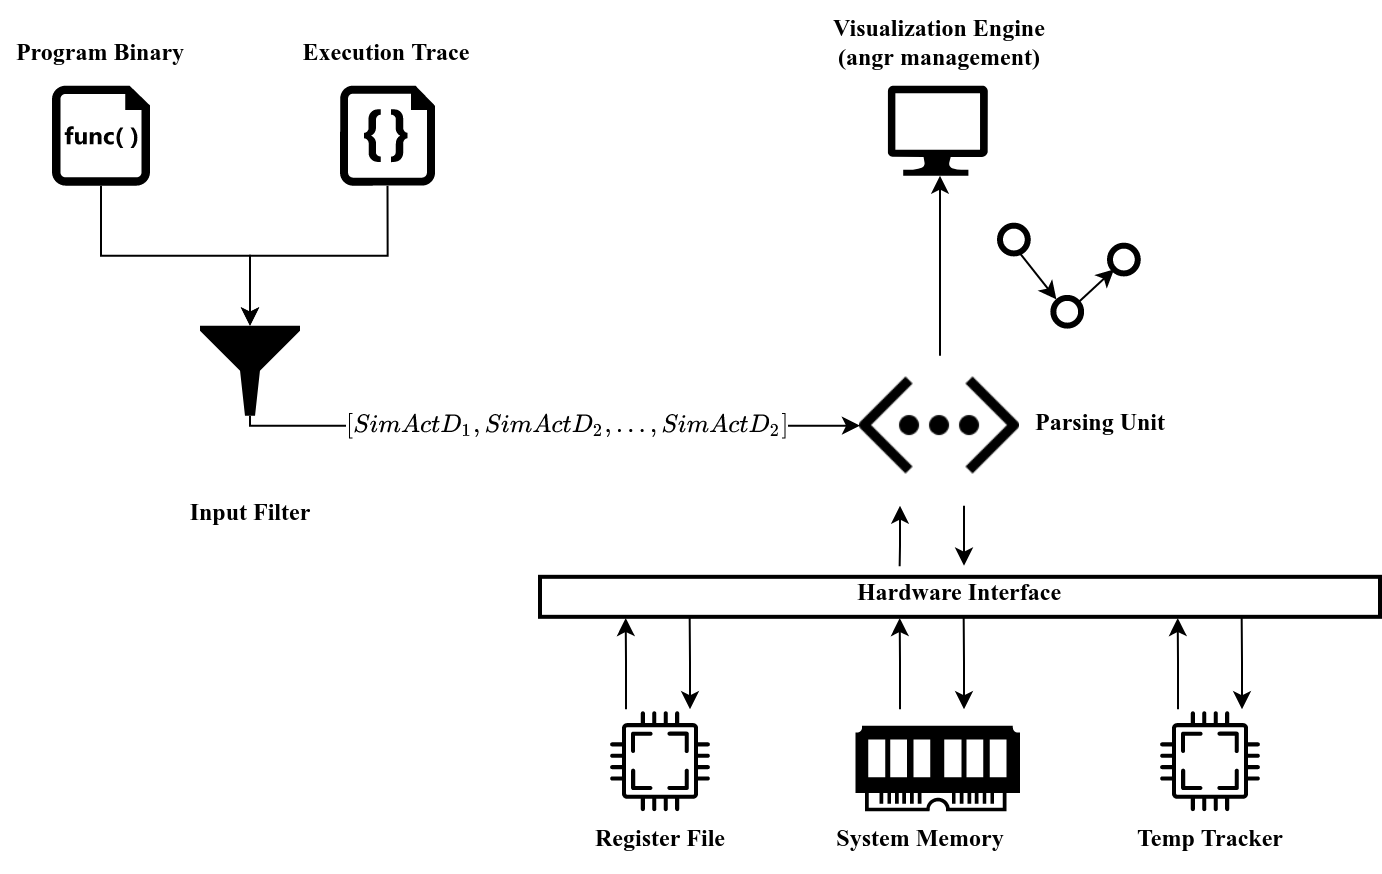
\includegraphics[width=0.8\linewidth]{images/design.png}
    \caption[Design Diagram]{Design diagram of proposed analysis.}
    \label{fig:design}
\end{figure}

The design goal of the proposed analysis is to ingest an arbitrary binary and execution trace and efficiently parse a representative data dependency graph for visualization. In order to develop this functionality, the design was split into the independent modules seen in Figure \ref{fig:design}.

\section{Input Filter}
This module is responsible for ingesting two critical files for data dependency graph generation: the program binary and the execution trace. The binary can be any executable file that the user would like to analyze while the execution trace must correspond to that binary. While execution trace generation was outside the scope of this thesis, the user could perform symbolic execution in \code{angr} upon the binary to generate it. This would typically involve creating the initial state at the first line of code that the user is interested in graphing and having the symbolic execution stop upon reaching the final line of code of interest. The resulting \code{SimState} must then be JSON encoded.

The input filter would then be responsible for decoding the execution trace to recover the underlying \code{SimState}. The only property of concern to this analysis within the \code{SimState} is its history, which contains an array of the read and write actions undertaken during symbolic execution. This array contains a series of \code{SimAction} instances, which may not all necessarily be concerned with the flow of data throughout the program's execution. The instances that belong to the \code{SimActionData} class are the only elements that concern data movement. Thus, this module will filter out all of the irrelevant elements from the history and output an array of the program's \code{SimActionDatas} in ascending order of the time in which they were taken.

\section{Parsing Unit}

\begin{figure}[hb]
    \centering
    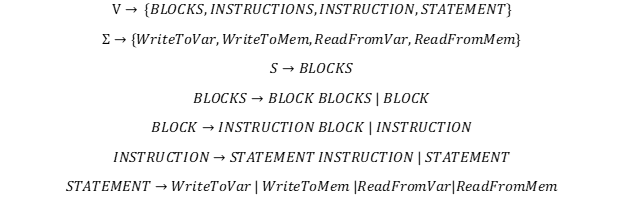
\includegraphics[width=0.8\maxwidth{\textwidth}]{cfg.png}
    \caption[Context Free Grammar of the Analysis' Language]{Context free grammar of the analysis' language. Designed to tightly mirror the aspects of \code{VEX IR} relevant to this analysis.}
    \label{fig:cfg}
\end{figure}

The parsing unit is the main module of the proposed analysis. 
I designed a context free grammar (Figure \ref{fig:cfg}) to capture the structure of the linear sequence of reads and writes ingested by the analysis. A recursive descent parser processes this sequence. This grammar follows the same structure of describing CPU actions that are taken by \code{VEX}. This design decision was driven by the fact that the grammar in question is relatively concise, and the code required to implement a recursive descent parser tightly mirrors the grammar \citep{redziejowski2007parsing}. Furthermore, the code that drives this analysis will need continued maintenance beyond the time frame of this thesis. Moreover, keeping the parser simpler and more readable, will make future contributions and improvements easier.

The terminals in the proposed context-free grammar  are used to represent the different categories of \code{SimActionData} that the analysis processes. As can be seen in the naming scheme of the terminals, a \code{SimActionData} is categorized based upon its action and type. The supported actions are WRITE and READ while the supported types are TMP, MEM, and REG. Although the MEM and REG types are straightforward, representing any operations that involve a memory address or register, the TMP type is not as readily apparent. TMP, short for temporary, operands can be viewed as variables as they are used to hold the result of intermediary steps in an operation. As an example, the AMD64 instruction \code{mov dword ptr [rbp – 0x4], 0x1d6} which moves the decimal value 470 into a memory offset from the base pointer, could be represented by the \code{SimActionDatas} presented in \ref{fig:tmp}. In this example, two temporary variables are used to hold the value of the base pointer register and the calculated offset from rbp to facilitate the memory write. 

\begin{figure}
    \centering
    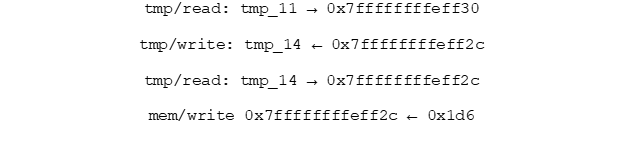
\includegraphics[width=0.8\maxwidth{\textwidth}]{tmp.png}
    \caption[Example of Temporary Operands in Angr]{Example of temporary operands in \code{angr}.}
    \label{fig:tmp}
\end{figure}

The largest unit that the analysis is concerned with is the block, with a program being a sequence of blocks. In \code{VEX}, a block is a collection of instructions with a single entrance and an unbounded number of exits. The end of a block is simply delineated by the \code{SimActionData} currently being parsed having a different block address from the next.

An instruction, while not being part of the \code{VEX} language, is incorporated into the analysis’ parser simply for readability. Rather than parsing the many statements that belong to a single block at a time, the statements belonging to a given instruction address are logically grouped. The end of an instruction is depicted by the \code{SimActionData} currently being parsed having a different instruction address from its successor. 

A statement is the smallest and most important unit of analysis, as \code{VEX} statements are what change state in the symbolic execution. A statement is parsed according to its type and action. It is during this portion of parsing where nodes in the data dependency graph are created and linked together.

The recursive descent parser is used to convert the provided sequence of \code{SimActionData} elements into a data dependency graph. The data dependency graph is then forwarded to the visualization engine for rendering a visualization to the screen.

\section{Hardware Interface}
This module serves as a supplementary module to the parsing unit, providing it with a memory of the read and write actions parsed thus far. This is imperative to have as, without tracking the reads and writes, it isn't possible to create edges between the nodes generated by the parser. The hardware interface facilitates the interactions between the parsing unit and the simulated register file, simulated system memory, and temporary tracker. The parsing unit can request to read from or write to a given register, variable, or memory address through the functionality it exposes.

In order to track the current state of all registers that the program moves data into and out of, an emulated register file is utilized to associate the register’s current value with its associated node in the graph. On a write to a register, the value and associated node are updated. On a read from a register, the current associated node is used as the value’s source for linking purposes. 

In order to track the current state of all memory addresses that the program reads and writes to, an emulated memory is also maintained. This works in the same manner as the register file. 

The temporary variable tracker is a per-block association of values with the current temporary node. This is reset at the end of a parsed block.

\section{Visualization Engine}
This module is responsible for ingesting the generated data dependency graph and visualizing it in an effective user interface for the binary analyst to peruse. This was accomplished through the creation of an \code{angr management} view.